%%%%%%%%%%%%%%%%%%%%%%%%%%%%%%%%%%%%%%%%%
% Simple Sectioned Essay Template
% LaTeX Template
%
% This template has been downloaded from:
% http://www.latextemplates.com
%
% Note:
% The \lipsum[#] commands throughout this template generate dummy text
% to fill the template out. These commands should all be removed when 
% writing essay content.
%
%%%%%%%%%%%%%%%%%%%%%%%%%%%%%%%%%%%%%%%%%

%----------------------------------------------------------------------------------------
%	PACKAGES AND OTHER DOCUMENT CONFIGURATIONS
%----------------------------------------------------------------------------------------

\documentclass[12pt]{article} % Default font size is 12pt, it can be changed here

\usepackage{geometry} % Required to change the page size to A4
\usepackage{subfigure}
\usepackage{tikz}
\usepackage{placeins}
\usetikzlibrary{arrows,snakes,backgrounds}
\geometry{a4paper} % Set the page size to be A4 as opposed to the default US Letter

\usepackage{graphicx} % Required for including pictures

\usepackage{float} % Allows putting an [H] in \begin{figure} to specify the exact location of the figure
\usepackage{wrapfig} % Allows in-line images such as the example fish picture

\usepackage{lipsum} % Used for inserting dummy 'Lorem ipsum' text into the template

\linespread{1.2} % Line spacing

%\setlength\parindent{0pt} % Uncomment to remove all indentation from paragraphs

\graphicspath{{./Pictures/}} % Specifies the directory where pictures are stored

\begin{document}

%----------------------------------------------------------------------------------------
%	TITLE PAGE
%----------------------------------------------------------------------------------------

\begin{titlepage}

    \newcommand{\HRule}{\rule{\linewidth}{0.5mm}} % Defines a new command for the horizontal lines, change thickness here

    \center % Center everything on the page

    \textsc{\LARGE University of Amsterdam}\\[1.5cm] % Name of your university/college

    \HRule \\[0.4cm]
    { \huge \bfseries The Hugin Project}\\[0.4cm] % Title of your document
    \HRule \\[1.5cm]

    \begin{minipage}{0.4\textwidth}
        \begin{flushleft} \large
            \emph{Author:}\\
            Inge \textsc{Becht} % Your name
        \end{flushleft}
    \end{minipage}

    {\large \today}\\[3cm] % Date, change the \today to a set date if you want to be precise

    %\includegraphics{Logo}\\[1cm] % Include a department/university logo - this will require the graphicx package

    \vfill % Fill the rest of the page with whitespace

\end{titlepage}

%----------------------------------------------------------------------------------------
%	TABLE OF CONTENTS
%----------------------------------------------------------------------------------------

\tableofcontents % Include a table of contents

\newpage % Begins the essay on a new page instead of on the same page as the table of contents 

%----------------------------------------------------------------------------------------
%	INTRODUCTION
%----------------------------------------------------------------------------------------

\section{Introduction} % Major section

When talking about reasoning with uncertainty an important part of it consists
of how to represent random variables that are dependable of other events when finding out
their likelihood. The Rule of Bayes shows this idea, but can be extended to the
bayesian model in which all events that are causally related are visualised with
their probabilities.

In this essay a bayesian network is constructed to show the basic idea of its
inner woking and to
show its prediction capabilities of a simplified problem (with only around 10
nodes). The subject of the
bayesian network consits of the question \emph{Will i be moving to a new
appartment?}. For the probabilitie assignment of the different events, a 2 year span is
kept in mindi, so that more precisely the question is \emph{Will I move to a
new appartment somewhere in the next two years?}. When assigning the values the noisy OR model (A way to assign
probabilitie values in a condition probability table) is used when possible
and else an explanation is given why it wouldn't make sense to use it. 
At the end the probability of me moving in the next two year are given with some
possible explanation for the outcome and some
experimentation with prior knowledge will show some more possible outcomes.

%------------------------------------------------


\section{Background information}

\subsection{The Bayesian network} % Sub-section

A Bayesian network is a model consisting of different nodes (the random
variables) in which each one
has a causal relation towards other nodes that it has a connection with. The
direction of the arrow shows the causal relation between two points.

A bayesian network has the following retraints in its construction:
\begin{itemize}
    \item The model should be acyclic. 
    \item All events should have a condition probability table 
    \item All nodes should have a causal relation towards another node
\end{itemize}

\begin{figure}[h]
    \begin{center}
        \tikzstyle{place}=[circle,draw=black,fill=white!20,thick]
        \tikzstyle{invis}=[circle,draw=white,fill=white,thick]
        \begin{tikzpicture}

            \node[invis] (critical) [] {};
            \node[place] (semaphore) [below of=critical] {C};
            \node[place] (leave critical) [right of=critical] {B};
            \node[place] (enter critical) [left of=critical] {A};
            \draw [arrows={->}] (enter critical.south) -- (semaphore.west);
            \draw [->] (leave critical.west) -- (enter critical.east);
            \draw [->] (leave critical.south) -- (semaphore.east);
        \end{tikzpicture}
        \caption{ A simple bayesian network}
        \label{ref:simple}\
    \end{center}
\end{figure}



Figure \ref{ref:simple} shows a very simple bayesian network. In this network
the outcome of A is dependable of B, and C is depended on both the probability
of A and B. Calculating
$\mu(A, B, C)$ can this way be simplified towards $\mu(C|A,B,)\mu(A|B)\mu(B)$.
As long as the probability tables are given the calculations become trivial.

\subsection{Noisy OR}
{
    Noisy OR is a way of distributing probability in conditional probability tables
    and makes the following assumptions:
    \begin{itemize}
        \item all causes are listed in the network for the event noisy OR is
            used on.
        \item Negated causes do not influence the effected event
        \item It is assued that Noisy OR only works in case 
    \end{itemize}
    In case an event $X$ has causes $A$, $B$ and $C$, the probability table will
    look as follows:

\FloatBarrier
\begin{centering}
    \begin{table}
        \begin{tabular}{|lll|ll|}
            \hline
            A & B & C & $\mu(X)$ & $\mu(\neg X)$ \\ \hline
            0 & 0 & 0 &   0      & 1\\
            0 & 0 & 1  &  $1 - \chi$  & $\chi$       \\ 
            0 & 1 & 0  &  $1 - \beta$ & $\beta$\\
            0 & 1 & 1  &  $1 - \beta\chi$ & $\beta \chi$\\       
            1 & 0 & 0  &  $1 - \alpha$ & $\alpha$     \\                     
            1 & 0 & 1  &  $1 - \alpha \chi$& $\alpha \chi$\\   
            1 & 1 & 0  &  $1 - \alpha \beta$&$\alpha \beta$ \\         
            1 & 1 & 1  &  $1 - \alpha \beta \ chi$  & $\alpha \beta \chi$ \\
            \hline
        \end{tabular}
        \caption{A Noisy OR example}
        \label{ref:money}
    \end{table}
\end{centering}



}

\section{Creating the network} % Sub-section

To create a network that predicts the chance of me moving in the next two years,
the first step was to consider the  direct possbile causes for this to happen. A
small set of the possible causes (that were used) are:

\begin{itemize}
    \item Money fluctuation:
        \begin{itemize}
            \item Earning more
            \item Earning less
            \item Earning the same
        \end{itemize}
    \item Noisy neighbours
    \item House becomes unlivable (by disasters 
\end{itemize}


\begin{figure}[h!]
    \centering
    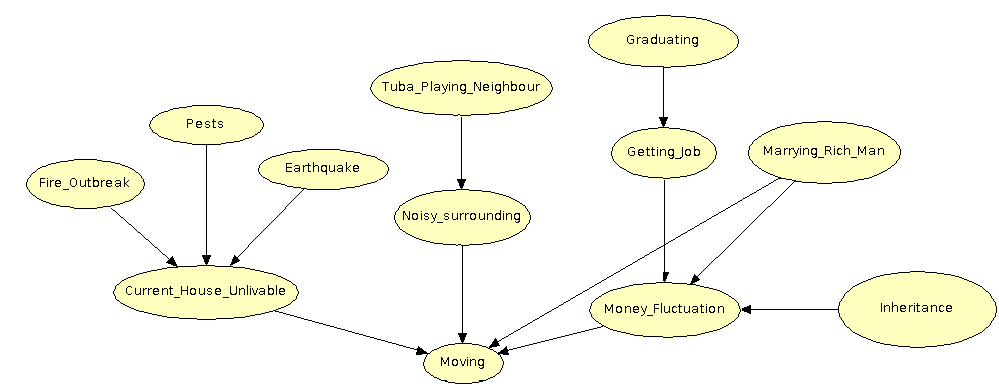
\includegraphics[width=1\textwidth]{network3}
    \caption{The completed network}
    \label{ref:complete}
\end{figure}
After this the causes of the these random variables were added to the network
until it consisted of approximately 10 nodes, as to be seen in
Figure \ref{ref:complete}: the completed network. The next sections will describe the
process and stuggles of adding the nodes to the network.

%------------------------------------------------

\subsection{Money fluctuation} % Sub-sub-section
Earning more money, as well as
less or the same amount, all influences if I will be able to afford to move or
afford paying the rent of my current appartment. This means that the node
can not be represented as just a single boolean probability. Alternatives are
to consider it as a causal three node structure (see left of figute
\ref{fig12}) or a single discrete node with three values (see right of figure \ref{fig12}).


\begin{figure}
    \centering
    \mbox{\subfigure[Money fluctuation
            considered as 3 causal boolean
        random variables]{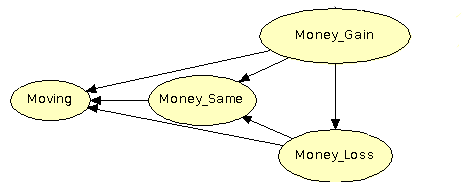
\includegraphics[width=3in]{booleanMoney.png}}\quad
        \subfigure[Money fluctuation considered
    as a discrete random variable]{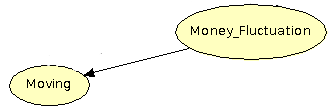
\includegraphics[width=2.5in]{3ValueMoney.png}}}
    \label{fig12}
\end{figure}


When using the 3 boolean nodes, it would be possible to implement noisy OR, but its downside
would be that it would create $2^3 = 8 $  dependencies towards the moving
node, which would assign much bigger complexity towards the bayesian network, as
well as create situations in which both \emph{money\_gain} and
\emph{money\_loss} are true in the probability tables,  which should have a zero
chance of happening and are thus irrelevant to the network \footnote{Although
    considering a two year span a situation like that could happen but would greatly
    complicate the idea of predicting the move and as such is not desired for this
simple example}.

Creating just one discrete node \emph{money\_fluctuation} gives only the
possibilty of \emph{high}, \emph{same} or \emph{low} being true when
considering the probability of moving, which makes the structure of the network
cleaner and less complicated. The only downside is that the probability
distribution of both moving and money fluctuation can not be made with Noisy Or
probability distribution as
its  use is only clear in case of boolean value distribution. The final choice
fell on using the single node to represent money.

\begin{figure}[h!]
    \centering
    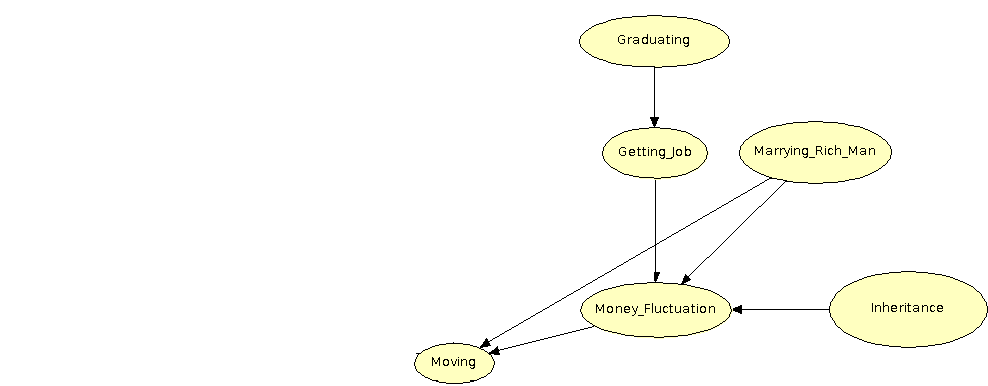
\includegraphics[width=1\textwidth]{network1}
    \caption{The completed network}
    \label{ref:money}
\end{figure}

\FloatBarrier
Figure \ref{ref:money} shows the causes that relate to money fluctuation. All
these nodes are boolean and give a high probability towards
\emph{money\_fluctuation} begin high when true. Only inheritance being true can
cause to decrease income (think about inheriting debt). Table
\ref{tab:singlebest} shows the probability of me graduating in the next two
years. As I am currently in the last year of my bachelor (and I am not
considering a masters degree) this probability is quite high. The esimation is
made by guesswork when considering how well I passed previous courses. Table
\ref{tab:twobest} shows the probability of marrying a rich man, which doesn't
seem to be very relevant in this time in life. Notice that marrying a rich man
has a direct causal relation to moving as well in \ref{ref:money}, as marrying would
probably require a bigger living area.
Table \ref{tab:threebest} shows the
possibility of me inheriting money.

\begin{table} 
    \centering
    \makebox[0pt][c]{\parbox{1.2\textwidth}{%
            \begin{minipage}[b]{0.5\hsize}\centering
                \begin{tabular}{ | c | c |}
                    \hline
                    & $\mu{(Graduating)}$ \\ \hline
                    1 & 0.8 \\ \hline
                    0 & 0.2 \\ \hline
                \end{tabular}
                \caption{Chance of graduating}
                \label{tab:singlebest}
            \end{minipage}
            \hfill
            \begin{minipage}[b]{0.5\hsize}\centering
                \begin{tabular}{ | c | c |}
                    \hline
                    & $\mu(Marrying\_rich\_man)$ \\ \hline
                    1 & 0.01\\ \hline
                    0 & 0.99 \\ \hline
                \end{tabular}
                \caption{Chance of marrying rich man}
                \label{tab:twobest}
            \end{minipage}
            \hfill
    }}
\end{table}


\begin{table}
    \centering
    \makebox[0pt][c]{\parbox{1.2\textwidth}{%
            \begin{minipage}[b]{0.5\hsize}\centering
                \begin{tabular}{ | c | c |}
                    \hline
                    & $\mu(Inheritance)$ \\ \hline
                    1 & 0.1 \\ \hline
                    0 & 0.9 \\ \hline
                \end{tabular}
                \caption{Chance of inheritance}
                \label{tab:threebest}
            \end{minipage}%
            \hfill
            \begin{minipage}[b]{0.5\hsize}\centering
                \begin{tabular}{ | c | cc|}
                    \hline
                    Graduating  & $\mu{(Job)}$  &$\mu(\neg Job)$\\ \hline
                    1 & 0.8 & 0.2 \\ \hline
                    0 & 0.2 & 0.8\\ \hline
                \end{tabular}
                \label{tab:fourbest}
                \caption{Chance of graduating}
            \end{minipage}
            \hfill
    }}
\end{table}

The probability of graduating, as seen in table \ref{fourbest} is determined by
me graduating. In case i graduate right now i believe the chance that I will get
a job quite high (still not a hundred percent because i might take two whole years
graduating or won't be able to find any work) and in case i don't graduate I will not be
looking for a job so it will be quite low.



\begin{centering}
    \begin{table}
        \begin{tabular}{|lll|lll|}
            \hline
            M & I & G & $\mu(more)$ & $\mu(same)$  & $\mu(less)$  \\ \hline
            0 & 0 & 0 &   0.1 & 0.6 & 0.3 \\
            0 & 0 & 1  &  0.8    & 0.2 & 0       \\ 
            0 & 1 & 0  &  0.1    & 0.85 & 0.05     \\
            1 & 0 & 0  &  0.9    & 0.1 & 0     \\                     
            0 & 1 & 1  &  0.8    & 0.1 & 0.1\\       
            1 & 0 & 1  &  1        & 0 & 0\\   
            1 & 1 & 0  &  0.9    & 0.1 & 0\\         
            1 & 1 & 1  &  0.99   & 0.01 & 0 \\
            \hline
        \end{tabular}
        \caption{Probability of money fluctuation}
        \label{ref:money}
    \end{table}
\end{centering}

\FloatBarrier
Table \ref{ref:money} shows the probabilities of earning more or less or the
same amount of money given getting married or inheriting or getting a job.
Although at first Noisy OR was only not used because of the discrete
\emph{money\_fluctuation} it now also becaoms apparent that noisy OR would not
work because there are possibly more causes for monery fluctuation than are
given right now.

%------------------------------------------------

\subsection{Adding noisy surroundings} 


\begin{figure}[h!]
    \centering
    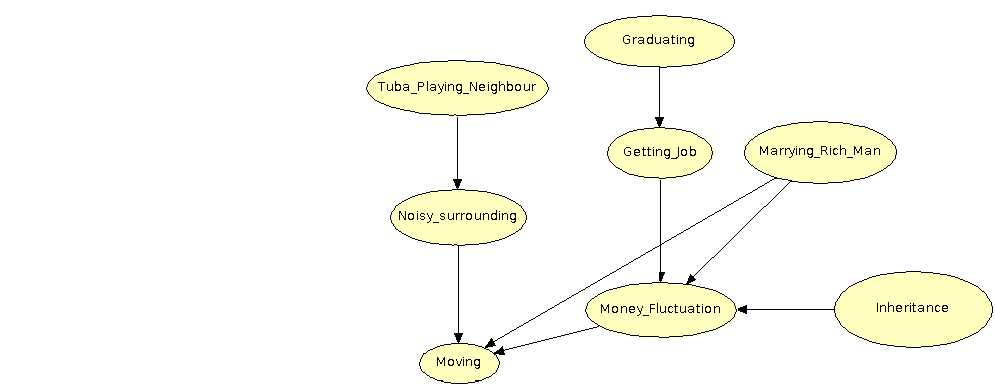
\includegraphics[width=1\textwidth]{network2}
    \caption{Adding the noisy surroundings node to the network}
    \label{ref:noisy}
\end{figure}

The second possible cause of moving is that the surroundings are too noisy. This
can happen because of multiple reasons, for instance the appartment is
located near a train track or because of neighbours that like to party (which
isn't all that uncommon for a student flat). There are a lot of
different possibilities to consider, so I kept it simple by adding just one possible event
of the tuba playing neihbour (see figure \ref{ref:noisy} ). This is quite a specific event to add to the
network and later some insight will be given in the consequences. Table
\ref{tab:tuba} shows the probability distribution of a possible tuba playing
neighbour and table \ref{tab:noise} shows the resulting probabilities for a
noisy surrounding. It should be clear that here the noisy OR distribution is not
applied as there are many other causes of a noisy surrounding that are not in
the network. Setting the change of a noisy surrounding 50-50 seems like the best
option as such a probability is quite hard to predict.

    \begin{table}
\centering
\makebox[0pt][c]{\parbox{1.2\textwidth}{%
    \begin{minipage}[b]{0.5\hsize}\centering
        \begin{tabular}{ | c | c |}
           \hline
           & $\mu(Tuba\_neighbour)$ \\ \hline
           1 & 0.02 \\ \hline
           0 & 0.98 \\ \hline
        \end{tabular}
        \caption{Chance of tuba playing neighbour}
        \label{tab:tuba}
    \end{minipage}%
   \hfill
    \begin{minipage}[b]{0.5\hsize}\centering
        \begin{tabular}{ | c | cc|}
           \hline
           Tuba  & $\mu{(Noise)}$  &$\mu(\neg Noise)$\\ \hline
           1 & 0.98 & 0.02 \\ \hline
           0 & 0.5 & 0.5\\ \hline
        \end{tabular}
        \caption{Chance of noisei}
        \label{tab:noise}
    \end{minipage}
    \hfill
}}
\end{table}


%----------------------------------------------------------------------------------------
%	MAJOR SECTION 1
%----------------------------------------------------------------------------------------

\subsection{Adding unlivable circumstances} % Major section


\begin{figure}[h!]
    \centering
    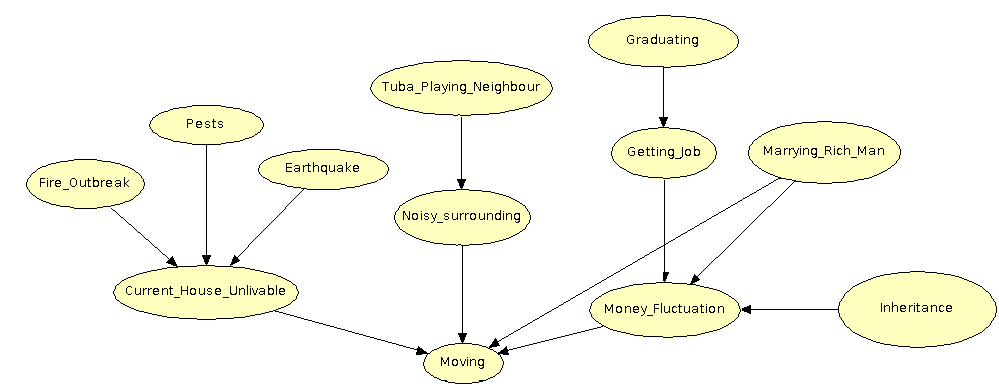
\includegraphics[width=1\textwidth]{network3}
    \caption{Adding the noisy surroundings node to the network}
    \label{ref:noisy}
\end{figure}

The last piece of the network consists of adding causes that make my current
appartment unlivable. A few things that I came up with were the outbreak of
fire(which has a quite low possibility of occurence but high chance of making a
living space unlivable), pests (a rather low
possibility although higher than fire), and an earthquake (quite possible that
it will happen, but a very very low chance of doing any serious damage).


\begin{table}
    \centering
    \makebox[0pt][c]{\parbox{1.2\textwidth}{%
            \begin{minipage}[b]{0.3\hsize}\centering
                \begin{tabular}{ | c | c |}
                    \hline
                    & $\mu{(Fire)}$ \\ \hline
                    1 & 0.01 \\ \hline
                    0 & 0.99 \\ \hline
                \end{tabular}
                \caption{Chance of fire}
                \label{tab:fire}
            \end{minipage}
            \hfill
            \begin{minipage}[b]{0.3\hsize}\centering
                \begin{tabular}{ | c | c |}
                    \hline
                    & $\mu(pest)$ \\ \hline
                    1 & 0.2\\ \hline
                    0 & 0.8 \\ \hline
                \end{tabular}
                \caption{Chance of pests}
                \label{tab:pests}
            \end{minipage}
            \hfill
            \begin{minipage}[b]{0.3\hsize}\centering
                \begin{tabular}{ | c | c |}
                    \hline
                    & $\mu(Earthquake)$ \\ \hline
                    1 & 0.3\\ \hline
                    0 & 0.7 \\ \hline
                \end{tabular}
                \caption{Chance of Earthquake}
                \label{tab:earthquake}
            \end{minipage}
    }}
\end{table}


\begin{table}
\begin{tabular}{|lll|ll|}
  \hline
  E & P & F & $\mu(U)$ & $\mu(\neg U)$   \\ \hline
  0 & 0 & 0 & 0 & 1 \\
  0 & 0 & 1  &  $0.6$       & $0.4$       \\ 
  0 & 1 & 0  &  $0.8$       & $0.2$       \\
  1 & 0 & 0  &  $0.001$     & $0.999$     \\                     
  0 & 1 & 1  &  $0.92$      & $0.4 * 0.2 =0.08$\\       
  1 & 0 & 1  &  $0.6004$    & $0.999 * 0.4 = 0.3996$\\   
  1 & 1 & 0  &  $0.8002$    & $0.999 * 0.2 = 0.1998$\\         
  1 & 1 & 1  &  $0.92008$   & $0.4 * 0.2 * 0.999 = 0.07992$ \\
  \hline
\end{tabular}
\caption{Probability of Unlivable conditions arising. 
        E = Earthquake, P = Pests, F = fire}
\label{tab:unlivable}
\end{table}

\FloatBarrier
The table that predicts the probability of unlivable house conditions makes use
of Noisy OR. The probability of a house being unlivable if there is no fire, no
pest and no earthquake in the two year span is considered so small that it can
be set to 0. This is not the most clean implementation, as a house could also
become unlivable by flooding. Instead of considering these chances too small to
matter, there could have been made a node \emph{Miscellaneous} under which all
other causes would fall. The making of the table without this
\emph{Miscellaneous} is shown in table \ref{tab:unlivable}. In case of both a
pest and a fire happening the probability will be much higher than for fire
alone and a bit higher than the probability for just pests, which does sound
quite likely. Setting the earthquake node on true if both pests and fire already
is almost does not make a different in the livabilty of the home, which is not
that surprising given the small probability created by 


%------------------------------------------------

\subsection{Combining all causes to predict moving probability} % Sub-section

Now that all other probabilities are known, the moving probability can be
calculated using the direct causes. A sample of all these 24 combinations is
shown in table \ref{moving}. Again these probabilities aren't calculated using
the noisy OR as moving is dependend of $Money_fluctuation$ and this is not a
boolean node. The choicie of moving or note is greatly dependend of the
\emph{money\_fluctuation} node. In case of only earning more or earning less
being true the
probabilities of moving are already quite high. All other events being true as
well only make the probability higher. In case that only earning the same is
true the chance of moving is very smalle and increases when other events are
true.

\begin{centering}
\small
\begin{table}
\begin{tabular}{|llll|ll|}
  \hline
  Marrying & Unlivable & Noisy & Money &  $\mu(Moving)$ & $\mu(\neg Moving)$   \\ \hline
  0 & 0 & 0 & L & 0.7 & 0.3 \\
  0 & 0 & 0 & S & 0 & 1 \\
  0 & 0 & 0 & H & 0.7& 0.3   \\
  0 & 0 & 1 & L & 0.5  & 0.5  \\ 
  0 & 0 & 1 & S & 0.1  & 0.9  \\ 
  0 & 0 & 1 & H & 0.7  & 0.3   \\ 
  0 & 1 & 0 & L & 0.8  & 0.2  \\ 
  0 & 1 & 0 & S & 0.85  & 0.15  \\ 
  0 & 1 & 0 & H & 0.9  &  0.1  \\ 
  \dots  &\dots   &\dots   &\dots   & \dots     &\dots \\
  1 & 0 & 1 & H & 0.9  & 0.1  \\ 
  1 & 1 & 0 & L & 0.9  & 0.1  \\ 
  1 & 1 & 0 & S & 0.95  & 0.05   \\ 
  1 & 1 & 0 & H & 0.95  & 0.05  \\ 
  1 & 1 & 1 & L & 0.9  & 0.1  \\ 
  1 & 1 & 1 & S & 0.99  & 0.01  \\ 
  1 & 1 & 1 & H & 1  & 0   \\ 
  \hline
\end{tabular}
\caption{The probability table of moving}
\label{moving}
\end{table}

\end{centering}

\subsubsection{Subsubsection 1} % Sub-sub-section


%------------------------------------------------

\subsubsection{Subsubsection 2} % Sub-sub-section


%------------------------------------------------

\subsubsection{The result} % Sub-sub-section
For these results Hugin lite was used with the network and probability table
inserted as stated as above.

\begin{centering}
\small
\begin{table}
    \begin{tabular}{|ll||}
        \hline
        Calculating probability of: &Priors & Probability    \\ \hline
        Moving  & - & 53.84 \\
        Getting Job & - & 68.00 \\
        Current House Unlivable & - & 16.53\\
        Noisy surrounding & - & 50.96
        Money Fluctuation(Higher) & - & 57.99\\
        Money Fluctuation(Same) & - & 32.62\\
        Graduating & Moving, Money\_fluctuation(High) & 91.45
        \hline
    \end{tabular}
\caption{Showing different kind of probability calculations that can be made
using the bayesian network.The first column is the event we like to calculate
the probability of. The priors column contains all events that are set
to true or false. The Probability column gives thecalculated probability  }
\label{probs}
\end{table}
\end{centering}

In \ref{probs}

Table \ref{probs} shows some different experimentations made with the final
bayesian network. The probability of moving without any priors seems quite
realistic with just above a 50 percent chance. Getting a job seems quite
realistic as well being just above three fifth. The 16 percent chance of my
house becoming unlivable seems rather high howerver whic probably has to do
mostly with the fact that a pest outbreak seems to have a high chance both in
occurence as in making the house unlivable (and it has happened before). The
noisiness of the surrounding is quite unpredictable with its 51 percent, a
consequence of only expending the network with the very unlikely \emph{Tuba
playing neighbour}


As I stated before only having the very specific node of \emph{tuba\_player}



\subsection{Conclusion}

Using a specific node like tuba player influences the \emph{Noisy\_surrounding}
node so little that it just comes down to the general 50-50 value.

It is quite hard to implement Noisy OR correctly on such a small network where
you try to simplify the model to implement. The
noisy OR could probabyl have been better applied when using very general boolean
nodes. When for instance considering the \emph{unlivable} node, better causes
would have been a categorization of different thinks like \emph{elemental
disasters} (which would combine e.g. flooding, fire and storms), and
\emph{infestation} (which woul cover e.g. pests and fungus).

%----------------------------------------------------------------------------------------
%	MAJOR SECTION X - TEMPLATE - UNCOMMENT AND FILL IN
%----------------------------------------------------------------------------------------

%\section{Content Section}

%\subsection{Subsection 1} % Sub-section

% Content

%------------------------------------------------

%\subsection{Subsection 2} % Sub-section

% Content

%----------------------------------------------------------------------------------------
%	CONCLUSION
%----------------------------------------------------------------------------------------

\section{Conclusion} % Major section


%----------------------------------------------------------------------------------------
%	BIBLIOGRAPHY
%----------------------------------------------------------------------------------------

\begin{thebibliography}{99} % Bibliography - this is intentionally simple in this template

    \bibitem[Figueredo and Wolf, 2009]{Figueredo:2009dg}
        Figueredo, A.~J. and Wolf, P. S.~A. (2009).
        \newblock Assortative pairing and life history strategy - a cross-cultural
        study.
        \newblock {\em Human Nature}, 20:317--330.

\end{thebibliography}

%----------------------------------------------------------------------------------------

\end{document}

